\documentclass[12pt,a4paper]{report}
\usepackage[utf8]{inputenc}
\usepackage[T1]{fontenc}
\usepackage[french]{babel}
\usepackage{geometry}
\geometry{top=2.5cm, bottom=2.5cm, left=2.5cm, right=2.5cm}
\usepackage{graphicx}
\usepackage{xcolor}
\usepackage{listings}
\usepackage{hyperref}
\usepackage{caption}
\usepackage{subcaption}
\usepackage{booktabs}
\usepackage{tabularx}
\usepackage{fancyhdr}
\usepackage{lmodern}

% Configuration des hyperliens
\hypersetup{
    colorlinks=true,
    linkcolor=blue,
    filecolor=magenta,      
    urlcolor=cyan,
    pdftitle={Rapport Technique StockMaster},
    pdfpagemode=FullScreen,
}

% Palette de couleurs pour la coloration du code
\definecolor{codeblue}{rgb}{0.13, 0.13, 1}
\definecolor{codegreen}{rgb}{0, 0.5, 0}
\definecolor{codered}{rgb}{0.9, 0, 0}
\definecolor{codebg}{rgb}{0.97, 0.97, 0.98}
\definecolor{primary}{RGB}{33, 150, 243} % Couleur principale StockMaster (Bleu Flutter)

% Configuration des listings de code (Dart & SQL)
\lstdefinelanguage{Dart}{
  keywords={abstract, any, as, assert, async, await, break, case, catch, class, const, continue, covariant, default, deferred, do, dynamic, else, enum, export, extends, extension, external, factory, false, final, finally, for, Function, get, hide, if, implements, import, in, infer, inline, inout, interface, is, late, library, mixin, new, null, of, on, operator, part, required, rethrow, return, set, show, static, super, switch, sync, this, throw, true, try, typedef, var, void, while, with, yield},
  sensitive=true,
  comment=[l]{//},
  morecomment=[s]{/*}{*/},
  string=[b]',
  morestring=[b]"
}

\lstset{
  backgroundcolor=\color{codebg},
  commentstyle=\color{codegreen},
  keywordstyle=\color{codeblue}\bfseries,
  numberstyle=\tiny\color{gray},
  stringstyle=\color{codered},
  basicstyle=\ttfamily\small,
  breakatwhitespace=false,         
  breaklines=true,                 
  captionpos=b,                    
  keepspaces=true,                 
  numbers=left,                    
  numbersep=5pt,                  
  showspaces=false,                
  showstringspaces=false,
  showtabs=false,                  
  tabsize=2
}

% Configuration des en-têtes et pieds de page
\pagestyle{fancy}
\fancyhf{}
\fancyhead[L]{StockMaster - Rapport Technique}
\fancyhead[R]{\leftmark}
\fancyfoot[C]{\thepage}
\renewcommand{\headrulewidth}{0.5pt}

\begin{document}

% ==========================================
% PAGE DE GARDE
% ==========================================
\begin{titlepage}
    \begin{center}
        
\includegraphics[width=0.25\textwidth]{logo.png}\\[1cm]
        {\large \textbf{ÉCOLE MAROCAINE DES SCIENCES DE L'INGÉNIEUR}}\\[0.2cm]
        {\large Filière Génie Informatique (2GInf)}\\[1.5cm]
        
        \rule{\linewidth}{1.5mm} \\[0.4cm]
        {\huge \bfseries StockMaster 📦 \\[0.3cm] \large Application Mobile ERP de Gestion de Stock Fluide} \\[0.2cm]
        \rule{\linewidth}{0.5mm} \\[1.5cm]
        
        {\large \textbf{Rapport de Projet de Fin de Module} \\[0.2cm] Développement d'une Application Mobile Autonome \& Sécurisée}\\[2cm]
        
        \begin{minipage}{0.45\textwidth}
            \begin{flushleft} \large
                \emph{Réalisé par :}\\
                \textbf{Anas HADDOU}\\
                \textbf{Alae Eddine MEHDI}
            \end{flushleft}
        \end{minipage}
        \hfill
        \begin{minipage}{0.45\textwidth}
            \begin{flushright} \large
                \emph{Encadré par :}\\
                \textbf{M. Samir BARA} (PhD, MCH)
            \end{flushright}
        \end{minipage}
        
        \vfill
        {\large Année universitaire : 2025/2026}
    \end{center}
\end{titlepage}

% Table des matières
\tableofcontents
\newpage

% ==========================================
% CHAPITRE 1 : INTRODUCTION
% ==========================================
\chapter{Introduction \& Contexte}

\section{La Problématique}
Dans le tissu économique actuel, les petites et moyennes structures (boutiques de détail, épiceries, garages de réparation, ateliers artisanaux) font face à un défi majeur : la gestion efficace et rigoureuse de leur inventaire. 
La majorité de ces commerces s'appuie encore sur des méthodes obsolètes et peu fiables :
\begin{itemize}
    \item \textbf{Cahiers de notes physiques :} Sujets aux pertes, aux ratures, aux oublis de saisie et à la dégradation physique.
    \item \textbf{Fichiers tableurs complexes (Excel) :} Souvent mal configurés, difficiles d'accès en mobilité et sujets à des erreurs de formules ou de doublons.
    \item \textbf{Absence de temps réel :} L'indisponibilité d'un historique structuré empêche toute anticipation des ruptures ou surstockages.
\end{itemize}

Ce manque de rigueur engendre des pertes financières directes dues aux invendus périmés ou obsolètes, et dégrade la satisfaction client lors de ruptures imprévues.

\section{La Solution : StockMaster}
\textbf{StockMaster} est né du besoin de fournir une solution moderne, autonome, sécurisée et ergonomique, accessible directement sur smartphone ou terminal mobile. L'application permet de centraliser la gestion des produits, de tracer chaque mouvement de stock et d'administrer précisément les accès utilisateurs selon une politique de rôles stricte.

Les objectifs clés assignés à cette application sont :
\begin{enumerate}
    \item \textbf{Centralisation :} Rassembler l'ensemble du catalogue produit (référence, description, prix d'achat, prix de vente, catégorie et fournisseur).
    \item \textbf{Traçabilité :} Enregistrer en temps réel chaque entrée et sortie de stock en indiquant qui a effectué l'action, quand, et pour quel motif.
    \item \textbf{Sécurité :} Garantir que seules les personnes autorisées puissent modifier le catalogue ou consulter les rapports financiers.
    \item \textbf{Autonomie (Offline-first) :} Pouvoir fonctionner entièrement en local, sans dépendance à une connexion internet constante, ce qui est crucial pour des entrepôts ou des zones de vente reculées.
\end{enumerate}

\section{Le Cycle de Vie du Projet}
Le développement de StockMaster a suivi un cycle méthodologique rigoureux, comprenant :
\begin{itemize}
    \item \textbf{Analyse des besoins :} Spécification fonctionnelle et cahier des charges.
    \item \textbf{Modélisation :} Conception de la base de données SQLite et architecture logicielle.
    \item \textbf{Développement :} Programmation en Flutter/Dart avec gestion de l'état réactive (Provider).
    \item \textbf{Optimisation \& Analyse :} Mise en place de scripts d'analyse de code pour mesurer la qualité structurelle.
    \item \textbf{Tests \& Validation :} Création de scénarios de validation pour chaque rôle applicatif.
\end{itemize}

\newpage

% ==========================================
% CHAPITRE 2 : ARCHITECTURE LOGICIELLE
% ==========================================
\chapter{Conception \& Architecture Technique}

\section{L'Architecture Logicielle (MVVM)}
Afin de garantir la séparation des responsabilités et la maintenabilité du code, l'application est structurée selon le patron d'architecture \textbf{MVVM (Model-View-ViewModel)}. Ce design s'aligne parfaitement avec la programmation déclarative de Flutter.

\begin{figure}[htbp]
    \centering
    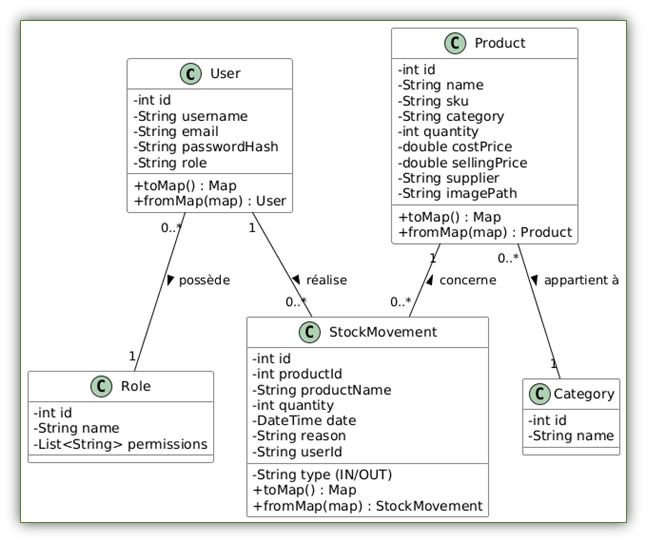
\includegraphics[width=0.85\textwidth]{diagClass.png}
    \caption{Diagramme UML de l'Architecture Applicative StockMaster}
    \label{fig:diag_uml}
\end{figure}

Les composants de l'architecture se déclinent ainsi :
\begin{itemize}
    \item \textbf{Model (Modèle) :} Représente les structures de données strictes (classes \texttt{Product}, \texttt{User}, \texttt{StockMovement}). Il s'agit de classes pures avec des méthodes de sérialisation JSON pour SQLite.
    \item \textbf{View (Vue) :} Composée des écrans (\texttt{login\_screen.dart}, \texttt{dashboard\_screen.dart}, etc.) programmés avec les widgets Flutter. Les vues observent les ViewModels et ne contiennent aucune logique métier complexe.
    \item \textbf{ViewModel (Modèle de Vue) :} Classe étendant \texttt{ChangeNotifier} (ex: \texttt{StockViewModel}, \texttt{AuthViewModel}). Il fait le pont entre la vue et la base de données. Lorsque le ViewModel effectue un traitement de données, il appelle \texttt{notifyListeners()} pour rafraîchir automatiquement l'interface utilisateur.
\end{itemize}

\section{Gestion d'État Réactive via Provider}
L'application utilise le package de gestion d'état \textbf{Provider} pour injecter les ViewModels au sommet de l'arbre des widgets et s'assurer que les écrans réagissent instantanément aux changements :
\begin{itemize}
    \item \texttt{AuthViewModel} : Centralise la session utilisateur, les tokens JWT simulés et le rôle actif.
    \item \texttt{StockViewModel} : Gère le catalogue, les alertes de stock critique et l'historique brut.
    \item \texttt{ThemeViewModel} : Gère la bascule à chaud entre le mode clair et le mode sombre.
    \item \texttt{LanguageViewModel} : Gère l'internationalisation dynamique de l'interface.
\end{itemize}

\section{Base de Données Relationnelle Embarquée (SQLite)}
Pour implémenter le concept \emph{Offline-first}, nous avons choisi \textbf{SQLite} via le package \texttt{sqflite}. Ce choix évite le recours à un serveur cloud obligatoire et assure des temps d'accès extrêmement rapides.
La base de données est initialisée à l'aide d'un pattern \emph{Singleton} dans la classe \texttt{DatabaseHelper}.

Voici la configuration détaillée des tables de \texttt{stockmaster.db} :

\begin{table}[htbp]
\centering
\caption{Schéma de la Table \texttt{products}}
\begin{tabularx}{\textwidth}{l l X}
\toprule
\textbf{Colonne} & \textbf{Type SQL} & \textbf{Description} \\
\midrule
\texttt{id} & INTEGER PK AUTOINCREMENT & Identifiant unique du produit. \\
\texttt{name} & TEXT NOT NULL & Nom ou désignation commerciale. \\
\texttt{sku} & TEXT NOT NULL & Code-barres ou référence unique d'inventaire. \\
\texttt{category} & TEXT NOT NULL & Catégorie d'appartenance. \\
\texttt{quantity} & INTEGER NOT NULL & Niveau actuel du stock physique. \\
\texttt{costPrice} & REAL NOT NULL & Prix unitaire d'achat. \\
\texttt{sellingPrice} & REAL NOT NULL & Prix de vente unitaire au client. \\
\texttt{supplier} & TEXT & Nom du fournisseur principal. \\
\texttt{images} & TEXT & Liste des chemins d'images (formaté en JSON). \\
\bottomrule
\end{tabularx}
\end{table}

\begin{table}[htbp]
\centering
\caption{Schéma de la Table \texttt{users}}
\begin{tabularx}{\textwidth}{l l X}
\toprule
\textbf{Colonne} & \textbf{Type SQL} & \textbf{Description} \\
\midrule
\texttt{id} & INTEGER PK AUTOINCREMENT & Identifiant utilisateur. \\
\texttt{username} & TEXT UNIQUE NOT NULL & Identifiant de connexion unique. \\
\texttt{email} & TEXT NOT NULL & Adresse mail de contact. \\
\texttt{passwordHash} & TEXT NOT NULL & Hachage cryptographique du mot de passe. \\
\texttt{role} & TEXT NOT NULL & Rôle de l'utilisateur (admin / employee). \\
\bottomrule
\end{tabularx}
\end{table}

\section{Sécurité Applicative et Gestion des Rôles (RBAC)}
La sécurité repose sur deux piliers majeurs :
\begin{enumerate}
    \item \textbf{Protection des identifiants :} Les mots de passe saisis par l'utilisateur ne sont jamais enregistrés en clair. Ils subissent un hachage unidirectionnel \textbf{SHA-256} à l'aide de la bibliothèque Dart \texttt{crypto} avant d'être insérés ou vérifiés dans la base de données.
    \item \textbf{Contrôle d'accès basé sur les rôles (RBAC) :} Le système possède deux tables dédiées, \texttt{roles} et \texttt{role\_permissions}, créant une association dynamique. L'UI masque ou désactive conditionnellement des sections critiques de l'application selon les droits de la session (ex: \texttt{hasPermission('view\_reports')}).
\end{enumerate}

\newpage

% ==========================================
% CHAPITRE 3 : PIPELINES & ANALYSE
% ==========================================
\chapter{Pipelines d'Analyse \& Outils d'Automatisation}

\section{Pipeline de Génération de Codes QR}
Pour l'intégration rapide de produits existants dans l'application, nous avons développé un pipeline d'automatisation Python utilisant la librairie \texttt{qrcode} (\texttt{generate\_qrs.py}). 
Ce script prend en entrée une liste de dictionnaires de produits contenant toutes les informations (SKU, nom, catégorie, quantité, prix, fournisseur), la convertit en chaîne JSON compacte sans espace, puis génère une image de code QR pour chaque produit dans le dossier \texttt{product\_qrs/}.

L'utilisateur peut alors scanner cette image directement avec la caméra de son mobile depuis l'écran de scanner de StockMaster, permettant un import ou une fiche produit instantanée.

\section{Pipeline d'Analyse Statique des Widgets (AST Parser)}
Pour mesurer la complexité de l'interface et documenter l'usage des composants graphiques, nous avons conçu un outil d'analyse statique écrit en Node.js (\texttt{tools/generate\_widgets\_report.js}). 
Ce script scanne récursivement le répertoire \texttt{lib/} et analyse chaque fichier Dart pour identifier l'utilisation des widgets système Flutter (ex: \texttt{Scaffold}, \texttt{ListView}, \texttt{TextFormField}) et des widgets personnalisés. 

Le script produit un rapport structuré \texttt{widgets\_report.json} regroupant les widgets par catégorie (Layout, Navigation, Inputs, Feedback, etc.) et par écran, qui est ensuite visualisé à travers une page Web HTML dynamique locale dans \texttt{docs/}.

\begin{figure}[htbp]
    \centering
    \includegraphics[width=0.85\textwidth]{rapport_statistics.png}
    \caption{Visualisation du Rapport de Widgets Flutter généré par le script Node.js}
    \label{fig:rapport_widgets}
\end{figure}

\section{Pipeline d'Importation et Traitement de Données (CSV/JSON)}
L'intégration de données en masse est gérée par le service \texttt{ImportService}. Le pipeline de traitement CSV comporte les étapes suivantes :
\begin{enumerate}
    \item \textbf{Détection d'encodage et normalisation :} Le fichier est lu en UTF-8 avec un repli automatique vers l'encodage Latin-1 en cas d'erreur de décodage. Les fins de lignes sont normalisées en \texttt{\textbackslash n}.
    \item \textbf{Détection automatique du séparateur :} Analyse de la première ligne pour déterminer si le délimiteur est une virgule (\texttt{,}) ou un point-virgule (\texttt{;}) couramment utilisé dans les fichiers CSV générés par Microsoft Excel en Europe.
    \item \textbf{Mappage intelligent des colonnes (Header Mapping) :} Utilisation de dictionnaires de synonymes pour associer des en-têtes divers (ex: \emph{Ref}, \emph{Barcode}, \emph{Code-barres}) à la variable standard \texttt{sku}.
    \item \textbf{Téléchargement et mise en cache des images :} Si le produit importé contient une URL d'image (commençant par http/https), le service effectue une requête réseau HTTP asynchrone, télécharge le fichier binaire de l'image, le sauvegarde dans le stockage local de l'application et enregistre son chemin d'accès local dans SQLite.
\end{enumerate}

\newpage

% ==========================================
% CHAPITRE 4 : EXTREITS DE CODE ET FONCTIONS
% ==========================================
\chapter{Implémentation \& Extraits de Code}

\section{Initialisation SQL et Gestion des Migrations (DatabaseHelper)}
La classe \texttt{DatabaseHelper} illustre l'usage du singleton et la configuration du schéma relationnel. Nous y gérons également le versionnage de la base de données avec des scripts de migration incrémentaux via \texttt{onUpgrade}.

\begin{lstlisting}[language=Dart, caption={Extrait de la classe DatabaseHelper}]
class DatabaseHelper {
  static final DatabaseHelper instance = DatabaseHelper._init();
  static Database? _database;

  DatabaseHelper._init();

  Future<Database> get database async {
    if (_database != null) return _database!;
    _database = await _initDB('stockmaster.db');
    return _database!;
  }

  Future<Database> _initDB(String filePath) async {
    final dbPath = await getDatabasesPath();
    final path = join(dbPath, filePath);
    // Version 8 pour activer les migrations incrementales
    return await openDatabase(
      path, 
      version: 8, 
      onCreate: _createDB, 
      onUpgrade: _onUpgrade
    );
  }

  Future _createDB(Database db, int version) async {
    await db.execute('''
    CREATE TABLE products (
      id INTEGER PRIMARY KEY AUTOINCREMENT,
      name TEXT NOT NULL,
      sku TEXT NOT NULL,
      category TEXT NOT NULL,
      quantity INTEGER NOT NULL,
      costPrice REAL NOT NULL,
      sellingPrice REAL NOT NULL,
      supplier TEXT,
      images TEXT
    )
    ''');
    // Creation des autres tables (users, movements, roles)...
    await _seedUsers(db);
    await _seedCategories(db);
    await _seedRolesAndPermissions(db);
  }
}
\end{lstlisting}

\newpage

\section{Algorithme d'Analyse du Fichier CSV (ImportService)}
Cet algorithme illustre la normalisation du flux de données CSV et le traitement robuste des types numériques lors de l'importation.

\begin{lstlisting}[language=Dart, caption={Algorithme de lecture et parsing CSV dans ImportService}]
  Future<Map<String, dynamic>> _importCsv(File file) async {
    try {
      String content;
      try {
        content = await file.readAsString(encoding: utf8);
      } catch (_) {
        content = await file.readAsString(encoding: latin1);
      }

      // Normalisation des retours a la ligne
      content = content.replaceAll('\r\n', '\n').replaceAll('\r', '\n');

      // Detection du delimiteur
      String delimiter = ',';
      final firstLine = content.split('\n').first;
      if (firstLine.contains(';') && !firstLine.contains(',')) {
        delimiter = ';';
      }

      final List<List<dynamic>> fields = const CsvToListConverter().convert(
        content,
        fieldDelimiter: delimiter,
        eol: '\n',
        shouldParseNumbers: true,
      );

      if (fields.isEmpty) return {'success': false, 'message': 'Fichier vide'};

      // Dictionnaire de synonymes pour le mappage d'en-tetes
      Map<String, String> columnMapping = {
        'nom': 'name', 'produit': 'name', 'product': 'name',
        'code': 'sku', 'ref': 'sku', 'reference': 'sku', 'barcode': 'sku',
        'quantite': 'quantity', 'qte': 'quantity', 'stock': 'quantity',
        'costprice': 'costPrice', 'achat': 'costPrice',
        'sellingprice': 'sellingPrice', 'prix': 'sellingPrice', 'vente': 'sellingPrice'
      };
      
      // Suite du traitement et insertion en base de donnees...
      return {'success': true, 'message': 'Importation reussie.'};
    } catch (e) {
      return {'success': false, 'message': 'Erreur CSV: $e'};
    }
  }
\end{lstlisting}

\newpage

\section{Authentification \& Session (AuthViewModel)}
Voici le modèle de vue gérant l'état de la session utilisateur ainsi que le hachage SHA-256 du mot de passe.

\begin{lstlisting}[language=Dart, caption={Gestion de connexion et session dans AuthViewModel}]
  Future<bool> login(String username, String password) async {
    _isLoading = true;
    notifyListeners();

    try {
      final user = await DatabaseHelper.instance.getUserByUsername(username);
      if (user == null) {
        _isLoading = false;
        notifyListeners();
        return false;
      }

      // Hachage du mot de passe et comparaison
      final inputHash = sha256.convert(utf8.encode(password)).toString();
      if (user.passwordHash == inputHash) {
        _currentUser = user;
        _permissions = await DatabaseHelper.instance.getPermissionsForRole(user.role);
        
        // Sauvegarde de session locale
        final prefs = await SharedPreferences.getInstance();
        await prefs.setString('username', user.username);
        await prefs.setString('role', user.role);
        await prefs.setString('email', user.email);

        _isLoading = false;
        notifyListeners();
        return true;
      }
    } catch (e) {
      debugPrint("Login error: $e");
    }

    _isLoading = false;
    notifyListeners();
    return false;
  }
\end{lstlisting}

\newpage

% ==========================================
% CHAPITRE 5 : RENDER VISUEL ET CAPTURES D'ECRAN
% ==========================================
\chapter{Galerie des Rendu Visuels \& Validation}

Ce chapitre présente les captures d'écran réelles issues de l'application mobile en cours d'utilisation sur émulateur et système physique.

\section{Écrans d'Authentification}
Le flux d'authentification comprend la connexion sécurisée, l'inscription et la récupération de mot de passe en cas d'oubli.

\begin{figure}[htbp]
    \centering
    \begin{subfigure}[b]{0.3\textwidth}
        \centering
        
\includegraphics[width=\textwidth]{login.jpeg}
        \caption{Écran de Login}
        \label{fig:login}
    \end{subfigure}
    \hfill
    \begin{subfigure}[b]{0.3\textwidth}
        \centering
        
\includegraphics[width=\textwidth]{register.jpeg}
        \caption{Création de Compte}
        \label{fig:register}
    \end{subfigure}
    \hfill
    \begin{subfigure}[b]{0.3\textwidth}
        \centering
        
\includegraphics[width=\textwidth]{forgotPA.jpeg}
        \caption{Oubli mot de passe}
        \label{fig:forgot_pass}
    \end{subfigure}
    \caption{Flux de Connexion et d'Enregistrement de l'Application}
\end{figure}

\section{Tableau de Bord \& Navigation Principale}
L'écran d'accueil offre des statistiques globales en cartes et intègre des visualisations d'alertes en cas de stock trop bas.

\begin{figure}[htbp]
    \centering
    
\includegraphics[width=0.4\textwidth]{Tableau_de_bord.png}
    \caption{Écran principal du Tableau de Bord (Dashboard) avec indicateurs}
    \label{fig:dashboard}
\end{figure}

\newpage

\section{Gestion du Catalogue Produit (CRUD)}
L'écran de catalogue permet d'afficher la liste des articles sous forme de cartes d'inventaire détaillées, avec une recherche textuelle intégrée.

\begin{figure}[htbp]
    \centering
    \begin{subfigure}[b]{0.45\textwidth}
        \centering
        
\includegraphics[width=0.9\textwidth]{products_list.png}
        \caption{Grille de Produits}
        \label{fig:products_grid}
    \end{subfigure}
    \hfill
    \begin{subfigure}[b]{0.45\textwidth}
        \centering
        
\includegraphics[width=0.9\textwidth]{prodcut_details.png}
        \caption{Détails d'un Produit}
        \label{fig:product_details}
    \end{subfigure}
    \caption{Catalogue et Vue détaillée de l'inventaire}
\end{figure}

L'ajout ou la mise à jour de produits s'effectue via un formulaire contenant la sélection de catégories et de fournisseurs.

\begin{figure}[htbp]
    \centering
    \begin{subfigure}[b]{0.45\textwidth}
        \centering
        
\includegraphics[width=0.9\textwidth]{add_product.png}
        \caption{Ajout d'un Produit}
        \label{fig:add_prod}
    \end{subfigure}
    \hfill
    \begin{subfigure}[b]{0.45\textwidth}
        \centering
        
\includegraphics[width=0.9\textwidth]{edit_product.png}
        \caption{Édition de Produit}
        \label{fig:edit_prod}
    \end{subfigure}
    \caption{Formulaires de Saisie de Données}
\end{figure}

\newpage

\section{Scanner de Codes QR \& Transactions}
L'application utilise le scanner intelligent via la caméra pour identifier directement le produit en magasin et journaliser les mouvements d'entrée ou de sortie dans la table d'historique.

\begin{figure}[htbp]
    \centering
    \begin{subfigure}[b]{0.45\textwidth}
        \centering
        
\includegraphics[width=0.9\textwidth]{codescanner.png}
        \caption{Scanner de QR Code}
        \label{fig:scan_qr}
    \end{subfigure}
    \hfill
    \begin{subfigure}[b]{0.45\textwidth}
        \centering
        
\includegraphics[width=0.9\textwidth]{transactions_history.png}
        \caption{Historique des Transactions}
        \label{fig:tx_history}
    \end{subfigure}
    \caption{Scanner et Tracé de l'historique des flux}
\end{figure}

\section{Export de Rapports Applicatifs}
Le module de reporting offre des fonctionnalités d'exportation vers des formats standards.

\begin{figure}[htbp]
    \centering
    \begin{subfigure}[b]{0.45\textwidth}
        \centering
        
\includegraphics[width=0.9\textwidth]{exported_as_pdf.png}
        \caption{Rapport Exporté en PDF}
        \label{fig:export_pdf}
    \end{subfigure}
    \hfill
    \begin{subfigure}[b]{0.45\textwidth}
        \centering
        
\includegraphics[width=0.9\textwidth]{exported_as_excel.png}
        \caption{Rapport Exporté en Excel}
        \label{fig:export_excel}
    \end{subfigure}
    \caption{Validation des fonctions d'export des données}
\end{figure}

\newpage

\section{Scénarios de Validation Applicative (Tests)}
Pour valider l'intégration complète et la sécurité du logiciel mobile, le tableau de tests de conformité suivant a été réalisé et validé.

\begin{table}[htbp]
\centering
\caption{Tableau de Validation des Cas de Test d'Intégration}
\begin{tabularx}{\textwidth}{l X l c}
\toprule
\textbf{Module} & \textbf{Action Testée} & \textbf{Comportement Attendu} & \textbf{Status} \\
\midrule
Sécurité & Connexion compte admin & Accès total au menu d'administration & \textbf{OK} \\
Sécurité & Connexion employé & Menu d'administration masqué et bloqué & \textbf{OK} \\
Mouvements & Enregistrement sortie & Stock réduit \& Ligne créée dans l'historique & \textbf{OK} \\
Importation & Fichier CSV mal formaté & Message d'erreur et rejet de la ligne & \textbf{OK} \\
Scanner & Scan QR code produit & Redirection directe vers la fiche produit & \textbf{OK} \\
\bottomrule
\end{tabularx}
\end{table}

\newpage

% ==========================================
% CHAPITRE 6 : CONCLUSION
% ==========================================
\chapter{Conclusion \& Perspectives}

\section{Bilan Réalisé}
Le développement de l'application \textbf{StockMaster} a permis de répondre avec précision aux besoins de modernisation des commerces de détail. Grâce à son fonctionnement autonome (offline-first) s'appuyant sur SQLite, l'application élimine toute contrainte réseau et préserve la confidentialité des données des commerçants.

Le patron d'architecture MVVM mis en place garantit une base de code propre, testable et évolutive. L'intégration de pipelines automatisés comme le parser de code pour les statistiques de widgets et la génération de QR codes montre une démarche industrielle rigoureuse dans la conception du produit.

\section{Perspectives d'Évolution (V2)}
Pour enrichir la solution, plusieurs évolutions techniques majeures sont envisagées :
\begin{enumerate}
    \item \textbf{Synchronisation Cloud Hybride :} Ajouter un service réseau périodique pour synchroniser la base SQLite locale avec un serveur central (API REST NestJS ou Firebase), permettant ainsi à un gérant de superviser plusieurs boutiques à distance en temps réel.
    \item \textbf{Version Web Multiplateforme :} Déployer une interface d'administration Web (Flutter Web ou React) destinée aux postes de travail PC pour faciliter les opérations de comptabilité et d'inventaire de masse.
    \item \textbf{Notification de Seuils Critiques :} Implémenter des notifications locales en arrière-plan lorsque la quantité d'un produit descend sous le niveau critique configuré.
    \item \textbf{Intégration de l'Intelligence Artificielle :} Ajouter un module d'analyse prédictive sur l'historique des mouvements pour aider le commerçant à anticiper la demande saisonnière et à optimiser sa trésorerie.
\end{enumerate}

\end{document}
